\section{Introduzione}

La meccanica respiratoria viene descritta in letteratura da numerosi modelli. Tra questi, un modello valido in determinate condizioni è rappresentato da un circuito RLC. Il modello permette di descrivere la meccanica respiratoria di un individuo sano. 

A partire dalle misure dell'indivuduo è possibile stimare i parametri per rappresentarlo tramite il modello stimato. Questo processo, sotto il nome di ottimizzazione parametrica, permette di adattare il sistema generale al caso specifico.

Nella seguente analisi viene affrontata la tecnica di identificazione parametriche tramite minimizzazione della differenza tra la risposta misurata e quella stimata.

Differenti tecniche di ottimizzazione permettono di stimare i parametri che permettono di descrivere il sistema considerato. 

Viene descritto sia il metodo di Nelder-Mead sia il metodo di Gauss-Newton, analizzandone punti in comune e differenze. Vengono fatte anche alcune considerazioni sulla convergenza del metodo e sul corretto condizionamento del problema.

\section{Background}

L'identificazione di sistemi è un insieme di tecniche che si prefigge lo scopo di identificare i parametri e il sistema tale da descrivere un certo fenomeno. La prima grande distinzione vede la separazione di due tecniche: identificazione parametrica e non parametrica. La prima parte stimando un modello del fenomeno e punta ad identificare i parametri che lo rappresentano. L'identificazione non parametrica, invece, procede senza conoscere il modello del fenomeno, al più ne stima alcune caratteristiche, e punta ad identificare il sistema che meglio lo descrive.

In questo caso si parte da un modello ben noto, un modello di meccanica polmonare lineare descritto da un circuito RLC, e se ne identificano i parametri descrittivi.

\subsection{Sistema RLC}

Il circuito RLC (\cref{fig:RLC}) permette, seguendo l'analogia elettrica, di descrivere un modello approssimato della meccanica respiratoria. Il modello prevedere una serie di resistenza, induttore e capacità. Sulla base dell'analogia tra la corrente elettrica e il flusso polmonare è possibile rappresentare, in un modello a parametri concentrati, le componenti di compliance e resistenza elastica dei polmoni \cite{ghafarian_review_nodate}. 

Questo modello permette di affrontare i casi fisiologici in cui il flusso entrante nei polmoni è predominante rispetto al flusso bloccato (flusso che invece aumenta notevolmente in caso di patologie ostruttive). L'analogia vede l'associazione della differenza di pressione alla differenza di potenziale, la corrente al flusso d'aria e l'induttanza come un'inertanza, ovvero la differenza di pressione richiesta per causare una variazione unitaria nel tasso di variazione del flusso nel tempo. 

In un caso paziente specifico sarebbero necessarie misure sperimentali così da ottenere il modello reale sul quale effettuare l'identificazione. In questo caso, non avendo a disposizione dati sperimentali, si utilizzano dei dati noti in letteratura \cite{khoo_physiological_2018}. 

\begin{itemize}
	\item $\operatorname{R}=0.1  \:\left[\text{cmH2O s}\over \text{L} \right]$
	\item $\operatorname{L}=0.01 \:\left[\text{cmH2O s}^2\over \text{L} \right]$
	\item $\operatorname{C}=0.1 \:\left[\text{L}\over \text{cmH2O} \right]$
\end{itemize}

In questo modello semplificato si considerano un'unica resistenza e un'unica compliance che vanno a rappresentare la complessiva e la capacità di accumulare aria del sistema respiratorio nel suo complesso. Quindi la resisitenza $\operatorname{R}$ porta con se il contributo resistivo delle vie aeree, dei tessuti polmonari e della parete toracica. La capacità $\operatorname{C}$ rappresenta il compliance dei tessuti e della parete toracica.

L'obiettivo è la predizione della pressione alveolare $p_A$ e della sua risposta dinamica a differenti forme d'onda di pressione applicare all'apertura delle vie aeree $p_{ao}$.

Applicando la prima legge di Kirchoff al circuito in \cref{fig:RLC} si ottiene:

\begin{equation}
p_{a O}=L \frac{d i}{d t}+R i+p_{a}
\end{equation}

Dove vale il legame:

\begin{equation}
	i=C \frac{d p_{a}}{d t}
\end{equation}

Da cui si ricava la funzione di trasferimento:

\begin{equation}
	H(s)=\frac{P_{a}(s)}{P_{ao}(s)}=\frac{1}{1+s R C+s^{2} L C}
\end{equation}

Questo mostra come $p_a$ è interamente dipendente da $p_{ao}$ e il sistema è un sistema con configurazione open-loop. 

\begin{figure}[b!]
	\centering
	\small{
	\def\svgwidth{0.8\linewidth}
	\input{lung_model.pdf_tex}}
	\caption{Astrazione di polmoni, parete toracica e spazio pleurico}
	\label{fig:model}
\end{figure}

\begin{figure*}[t]
	\begin{subfigure}{0.5\linewidth}
		\centering
		 	\small{\def\svgwidth{0.85\linewidth}
	\input{RLC.pdf_tex}}
	\caption{}
	\end{subfigure}\hfill
	\begin{subfigure}{0.5\linewidth}
		\centering
	\def\svgwidth{0.8\linewidth}
	\input{RLC_tf.pdf_tex}
	\caption{}
\end{subfigure}
\caption{Circuito RLC rappresentante la meccanica polmonare (a); sistema open loop rappresentante il circuito RLC (b)}
\label{fig:RLC}
\end{figure*}

\subsection{Identificazione dei parametri}

Non avendo a disposizione dati paziente specifici sulla meccanica respiratoria i dati verranno generati tramite la procedura \texttt{rlc\_fun.m} che restituisce la risposta del circuito RLC fornendogli in ingressi i parametri del sistema. 

A questo può essere aggiunto anche del rumore.

\subsection{Algoritmo di Nelder–Mead}

Una volta assunto come modello del sistema la funzione di trasferimento di un circuito RLC, per stimare i parametri è necessario definire una funzione obiettivo. Tale funzione rappresenta la differenza tra la risposta misurata (vera) del sistema e quella stimata:

\begin{equation}
\underline e=\underline y^{\operatorname{pred}} - \underline y^{\operatorname{mis}}
\end{equation}

E la ricerca dei parametri corretti punta alla minimizzazione della funzione obiettivo definita come:

\begin{equation}
 \mathrm{E}={1\over 2} \|\underline e\|^2
 \label{eq:obj}
\end{equation}

Uno dei possibili modi per affrontare questo problema consiste nell'affidarsi alla routine di \texttt{Matlab} nota come \texttt{fminsearch()}. Tale procedura si occupa di restituire i parametri ottimali. In particolare, questa funzione sfrutta l'algoritmo di Nelder Mead \cite{lagarias_convergence_1998}. Tale metodo non fa uso di derivate e si basa sul concetto di un simplesso approssimando il punto di ottimo locale in $n$ variabili. 


\subsection{Metodo di Gauss-Newton}

Un'alternativa è il metodo di Gauss-Newton. Il metodo, diversamente dal precedente, richiede di portare in conto anche le derivate. 

La minimizzazione dell'\cref{eq:obj} è un problema non lineare ai minimi quadrati. La soluzione numerica sfrutta il metodo di Gauss Newton. Come il metodo di Newton, si impone la stazionarietà, condizione che si riflette sulla j\textsuperscript{ma} compnente:

\begin{equation}
	(\nabla \mathrm {E})_{j}=\sum_{k} e_{k} \cdot \frac{\partial e_{k}}{\partial p_{j}}
\end{equation}

Ovvero tale differenziazione corrisponde a premoltiplicare per la matrice di sensibilità J:
\begin{equation}
\nabla \mathrm{E}=\underline{\underline{J}}^{T} \underline{e}
\end{equation}

Utilizzando quindi l'algoritmo di Newton l'iterazione al passo $k+1$ cercherà i parametri ($\underline p$) come:
\begin{equation}
\underline{p}^{(k+1)}=\underline{p}^{(k)}-\left.[\nabla \left(\nabla \mathrm E\right)]^{-1} \left(\nabla \mathrm E \right)\right|_{\underline{p}^{k}}	
\end{equation}

Per l'approssimazione introdotta da Gauss \cite{nocedal_numerical_2006} è possibile trascurare le componenti quadratiche dovute alla derivata seconda: 

\begin{equation}
	\begin{aligned}
	(\nabla^2 \mathrm{E})_{i j}=\frac{\partial \mathrm{E}}{\partial p_{j} \partial p_{j}}&=\frac{\partial}{\partial p_{i}}\left(e_{k} \frac{\partial e_{k}}{\partial p_{j}}\right)\\&=\frac{\partial e_{k}}{\partial p_{i}} \frac{\partial e_{k}}{\partial p_{j}}+\cancel{e_{k} \frac{\partial^{2} e_{k}}{\partial p_{j} \partial p_{i}}}	
	\end{aligned}	
\end{equation}

Ovvero considerare l'iterazione semplicemente come:

\begin{equation}
\underline{p}^{(k+1)}=\underline{p}^{(k)}+\underline h^{(k)}
\end{equation}

Dove l'incremento sarà:

\begin{equation}
\underline h^{(k)}=-\left.\left[\underline{\underline{J^{T}}} \:\underline{\underline{J}}\right]^{-1} \cdot \underline{\underline{J}}^{T} \underline{\underline{e}}\right|_{\underline{p}}(k)
\end{equation}


\begin{figure*}
	\begin{subfigure}{0.25\linewidth}
		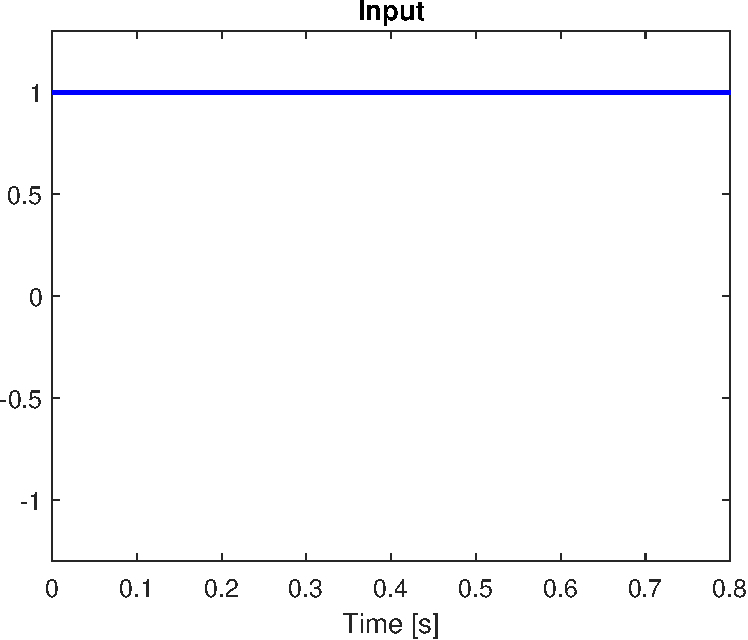
\includegraphics[width=0.9\linewidth]{step}
		\caption{}
	\end{subfigure}\hfill
	\begin{subfigure}{0.25\linewidth}
		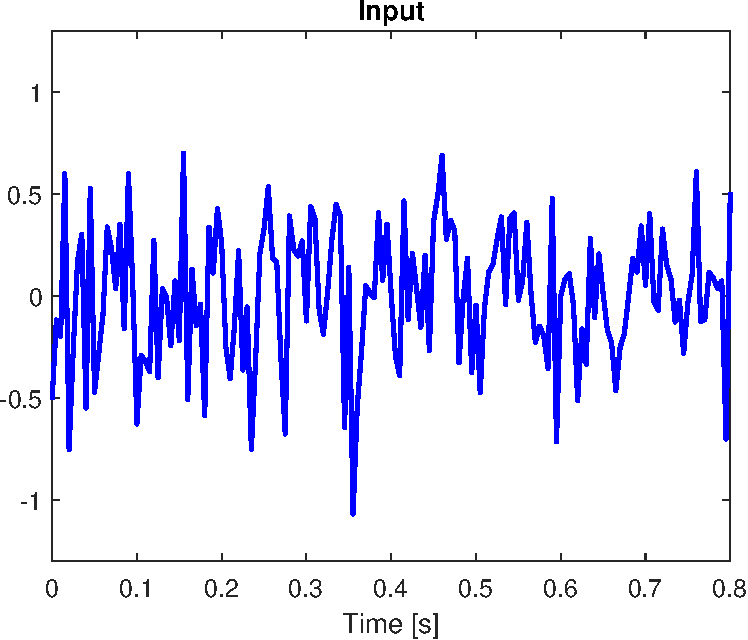
\includegraphics[width=0.9\linewidth]{rgs}
		\caption{}
	\end{subfigure}\hfill
	\begin{subfigure}{0.25\linewidth}
		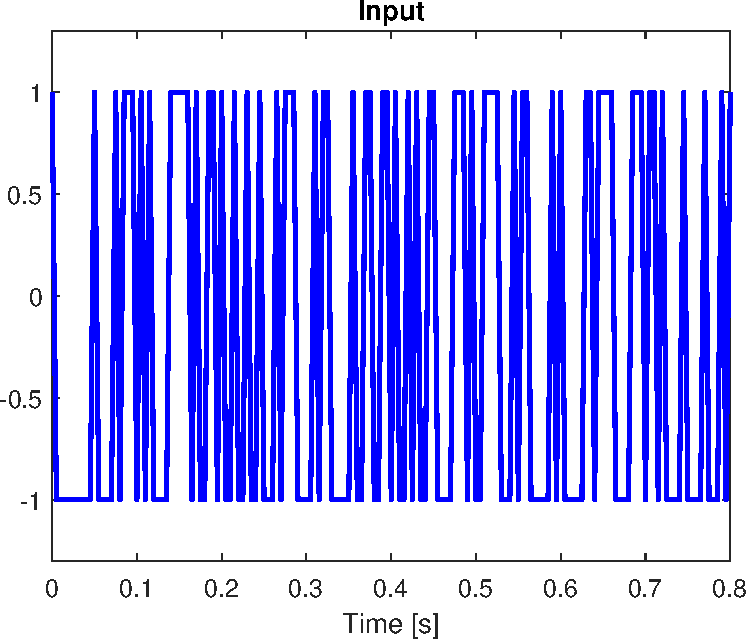
\includegraphics[width=0.9\linewidth]{rbs}
		\caption{}
	\end{subfigure}\hfill
	\begin{subfigure}{0.25\linewidth}
		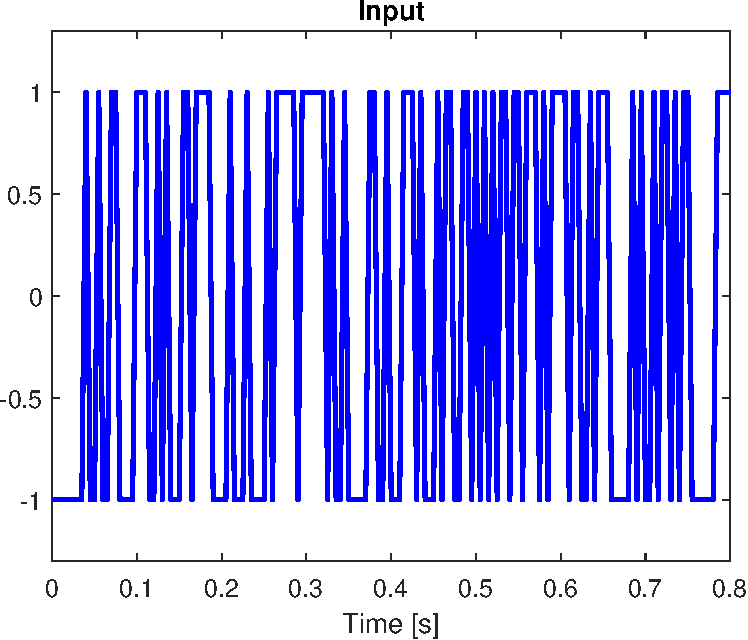
\includegraphics[width=0.9\linewidth]{prbs}
		\caption{}
	\end{subfigure}\hfill
	\caption{Differenti ingressi utilizzati per stimolare il sistema RLC. Ingresso a gradino (a); ingresso di tipo binario random (b); segnale gaussiano random (c); segnale binario pseudorandomico (d). I segnali sono stati generati tramite il comando \texttt{idinput()} appositamente per l'identificazione di sistemi \cite{idinput}.}
	\label{fig:inputs}
\end{figure*}


\section{Metodi}

Dunque il problema di identificazione parametrica viene affrontato come un problema di minimizzazione che porta a trovare i parametri ottimali. Sono quindi riportate le due differenti analisi.


\subsection{Minimizzazione}

Nel primo metodo si utilizza la routine di \texttt{Matlab} \texttt{fminsearch()}. La risposta vera del sistema viene calcolata tramite la routine \texttt{rlc\_fun.m} che si occupa, una volta fornitegli i coefficienti $R,\:L,\:C$ e l'ingresso, la risposta del sistema dinamica. Una volta generati i dati corrispondenti alla risposta vera del sistema è possibile procedere all'ottimizzazione. 

Si richiama allora la procedura \texttt{fminsearch()} fornendogli la funzione obiettivo, il punto iniziale e le variabile necessarie per il calcolo della funzione obiettivo (ingresso e discretizzazione temporale). La funzione obiettivo è presente all'interno della routine \texttt{onj\_fun.m} e si occupa di fare la differenza tra l'uscita vera e quella predetta. L'uscita predetta viene calcolata ad ogni iterazione sfruttando la procedura di \texttt{rlc\_fun.m} andando a calcolare la risposta del sistema RLC con i parametri aggiornati di volta in volta mediante l'algoritmo di Nelder-Mead. 

Effettuando un primo test, con rumore gaussiano, è possibile stimare i parametri. 

Inoltre, è possibile estrarre alcune informazioni dal processo di ottimizzazione. In particolare, si vede come nonostante la risposta del sistema viene stimata correttamente (\cref{fig:primo_test_4_parametri}), l'errore sui parametri è piuttosto alto (\cref{tab:test_3_param}).

\begin{table}[bt]
\begin{tabular}{|c|c|c|c|c|}
	\hline
	& Vero & Iniziale & Stimato & Errore relativo \\
	\hline
	$R$ & 0.100 & 0.150 & 0.119 & 0.197 \\
	\hline
	$L$ &  0.010 & 0.008 & 0.012 & 0.206 \\
	\hline
	$C$ & 0.100 & 0.280 & 0.083 & 0.169 \\
	\hline
\end{tabular}
\caption{Risultati dell'ottimizzazione con \texttt{fminsearch()} considerando 3 parametri.}
\label{tab:test_3_param}
\end{table}

\begin{figure}[bt]
	\centering
	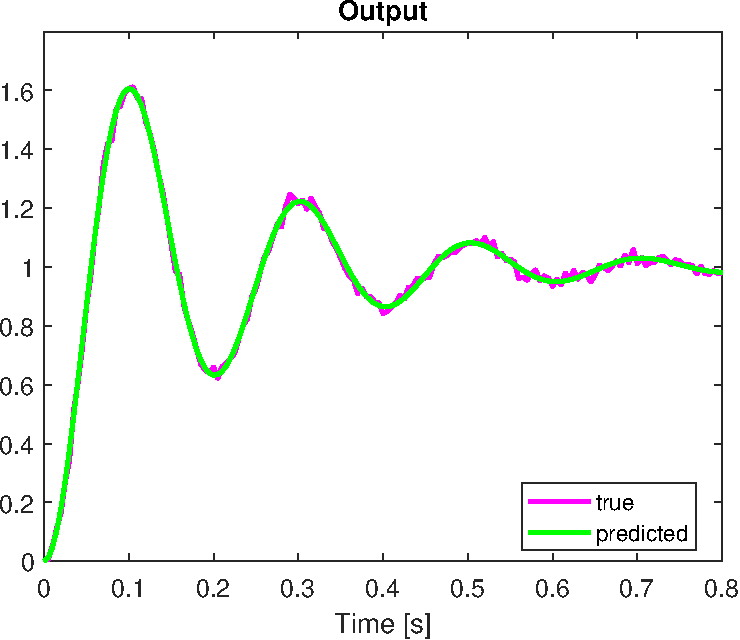
\includegraphics[width=\linewidth]{primo_test_4_parametri}
	\caption{Confronto tra la risposta vera (con aggiunta di rumore gaussiano) e la risposta stimata dopo aver ottimizzato i parametri (caso iniziale con 3 parametri). La risposta viene stimata correttamente e la procedura di stima va ad effettuare una sorta di filtraggio del rumore.}
	\label{fig:primo_test_4_parametri}
\end{figure}

\subsection{Non identificabilità strutturale}

Il problema, per come è stato posto, presenta una formulazione sbagliata. Infatti, andando a calcolare la matrice di sensibilità si vedono alcuni problemi. La matrice di sensibilità non è altro che l'insieme delle derivate della misura n\textsuperscript{ma} rispetto al j\textsubscript{mo} parametro. Calcolando quindi numericamente lo Jacobiano è possibile fare alcune considerazioni. 
Per calcolarlo è sufficiente perturbare rispetto al j\textsuperscript{mo} parametro e calcolarne la derivata come rapporto incrementale tra la risposta del sistema con ingresso perturbato e lo stato non perturbato rispetto la perturbazione:
\begin{equation}
	J_{i}={y_{\operatorname{pert}}-y_{\operatorname{ref}}\over |\operatorname{pert_i}|}
	\label{eq:J}
\end{equation}

I risultati numerici mostrano come la matrice ha un numero di condizionamento molto alto $1.856 \:10^7$ ma sembrerebbe avere rango massimo. Tuttavia, andando ad indagare i valori singolari si vede come uno dei tre è in realtà molto piccolo, abbastanza da poter essere considerato numericamente nullo. Nonostante il software percepisce un numero diverso da zero questo è in realtà nullo ed indica come nel problema c'è una dipendenza tra i parametri.

Questo è legato al fatto che nella risposta di trasferimento in realtà i parametri sono soltanto due, dati dal prodotto dei tre valori numerici legati ai componenti circuitali:
\begin{equation}
	\begin{aligned}
		\theta_1&=LC\\
		\theta_2&=RC
	\end{aligned}
\end{equation}

\subsection{Parametri ottimi}

Considerando quindi il problema nella sua versione ben condizionata è possibile procedere a stimare i parametri $\theta_1$ e $\theta_2$. 
In particolare è possibile analizzare il risultato ottenuto considerando diversi ingressi, mostrati in \cref{fig:inputs}.

Per farlo viene riorganizzato il codice in modo da racchiudere la generazione dei dati e l'ottimizzazione in due procedure che possono essere richiamate di volta in volta con i differenti ingressi. Con tutti gli ingressi testati l'errore rimane sotto il 2\% pur mantenendo una certa variabilità tra le differenti iterazioni. 

\begin{figure}[bt]
	\centering
	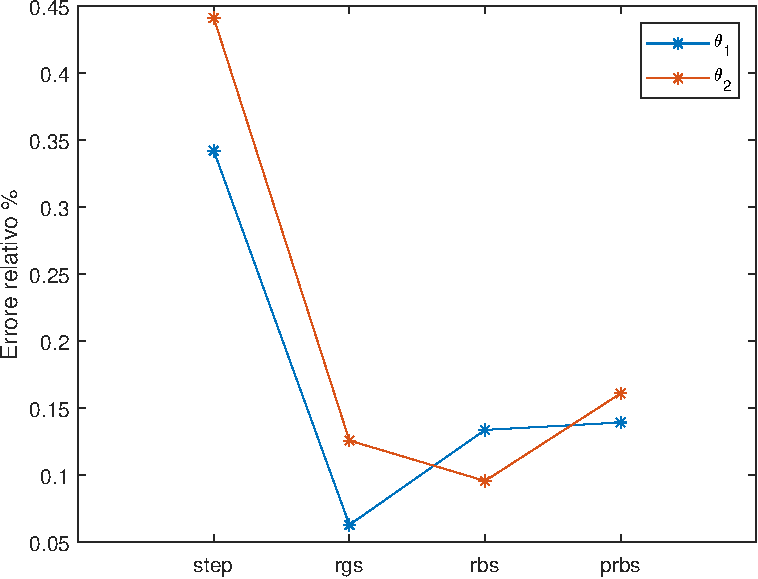
\includegraphics[width=0.95\linewidth]{error}
	\caption{Errore sui due parametri con i differenti segnali di ingresso utilizzati. Tra differenti ripetizioni dell'algoritmo l'errore potrebbe variare (sia a causa del metodo che della randomicità degli ingressi)}
\end{figure}

\subsection{Gauss Newton}

Un approccio differente prevede l'utilizzo dell'algoritmo di Gauss Newton. Si cerca la minimizzazione della funzione obiettivo per il tramite dell'iterazione in \cref{eq:obj}. 

È necessario calcolare, per procedere lungo le iterazioni, lo Jacobiano. Questo viene calcolato tramite la routine \texttt{jacobian\_fun.m}. Tale routine prende in ingresso il vettore dei parametri, l'ingresso e il vettore dei tempi e si occupa di calcolare la derivata numerica delle misure (risposta stimata) rispetto al parametro. Per farlo va a perturbare la j\textsuperscript{ma} componente della risposta facendo riferimento al j\textsuperscript{mo} parametro e ne calcola il rapporto incrementale. La procedura è analogo a quanto espresso per la matrice di sensibilità nell'\cref{eq:J}. 

È possibile sfruttare gli stessi ingressi del caso precedente (\cref{fig:inputs}). I risultanti seguenti fanno riferimento ad un ingresso tipo gradino. 

\begin{figure*}[bt]
	\begin{subfigure}{0.5\linewidth}
			\centering
		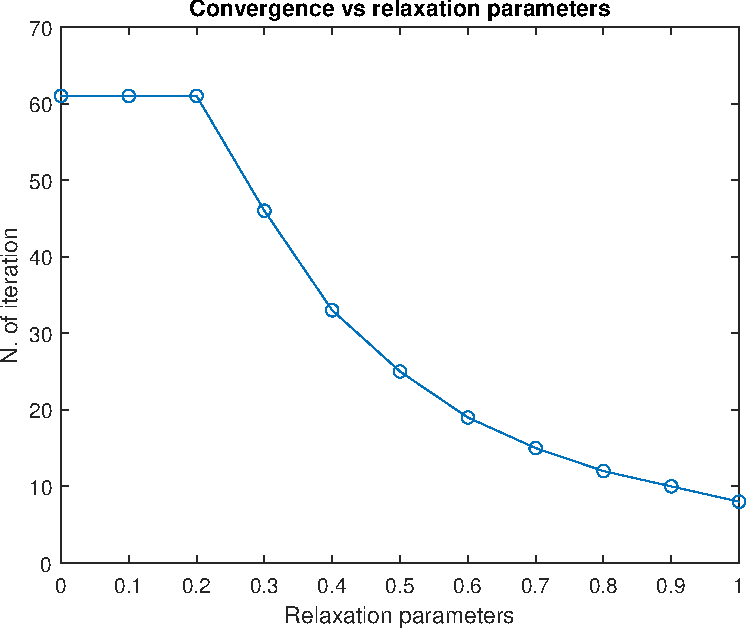
\includegraphics[width=0.85\linewidth]{convergence_vs_relaxation}
		\caption{}
	\end{subfigure}\hfill
	\begin{subfigure}{0.5\linewidth}
			\centering
		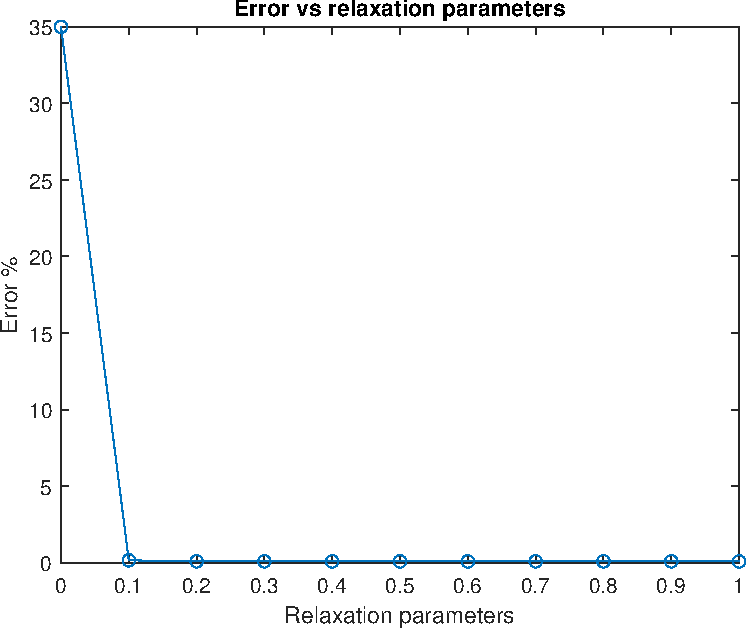
\includegraphics[width=0.85\linewidth]{error_vs_relaxation}
		\caption{}
	\end{subfigure}
	\caption{Effetto del parametro di rilassamento sul metodo di Gauss-Newton. In (a) si vede come più il parametro è piccolo più il metodo converge lentamente.}
	\label{fig:relaxation}
\end{figure*}

\begin{figure}[bt]
	\centering
	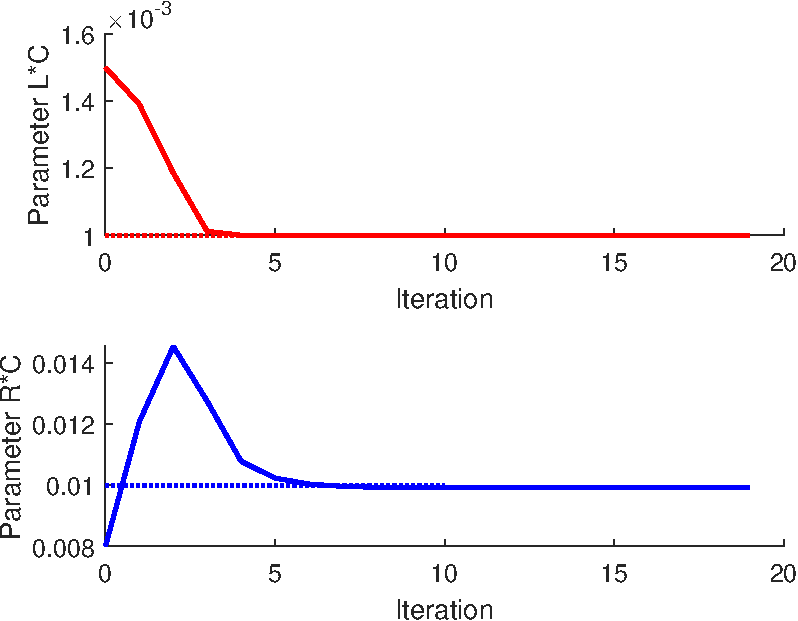
\includegraphics[width=0.9\linewidth]{gaussnewton}
	\caption{Metodo di Gauss Newton arrivato a convergenza con 19 iterazioni, $\alpha=0.6$, $\lambda=0.1$. In tratto continui i valori aggiornati durante le iterazioni, linea tratteggiata per i valori veri (obiettivo di minimizzazione).}
\end{figure}



Per aiutare il metodo a convergere si aggiunge un parametro di rilassamento ($\alpha$) che permette di modulare l'incremento tra un'iterazione e la successiva:
\begin{equation}
\underline{p}^{(k+1)}=\underline{p}^{(k)}+\alpha^{(k)} \underline{h}^{(k)}
\end{equation}

Introducendo invece parametro di regolarizzazione $\lambda >0$ si ottiene sempre l'inversione di una matrice non singolare \cite{nocedal_numerical_2006} e si evitano problemi di cattivo condizionamento. 

\begin{equation}
\left[\underline{\underline{J^{T}}} \underline{J}\right]^{-1} \longrightarrow \left[\underline{\underline{J}}^{T} \underline{\underline{J}}+\lambda^{(k)} \underline{\underline{I}}\right]^{-1}
\end{equation}



Il problema ricade sulla scelta del parametro ottimo, se troppo grande può rovinare la velocità di convergenza del metodo mentre se troppo vicino allo zero può essere inefficiente e portare verso le singolarità dello Jacobiano. 

Fissando il numero di iterazioni massimo è possibile confrontare come varia la convergenza (tempo di convergenza) al variare dei parametri di rilassamento e di regolarizzazione (\cref{fig:relaxation}). Si considera il tempo di convergenza come il numero di passi necessari ad avere una soluzione valida, soluzioni tali da non dare il risultato entro il numero di passi fissati vengono considerate non convergenti.

Per il parametro di regolarizzazione non si ottengono miglioramenti in quanto il problema è già ben condizionato. Per il parametro di rilassamento invece si vede fortemente la sua influenza sulla velocità di convergenza del metodo. 

Una notevole importanza è ricoperta anche dal punto iniziale. 
Le tecniche utilizzate finora considerano il punto iniziale come una quantità ottenuta scaldando i parametri reali con i seguenti fattori:
\begin{equation}
	\begin{aligned}
		&\theta_1^{0}=1.5\cdot \theta_1\\
		& \theta_2^{0}=0.8\cdot \theta_2
	\end{aligned}
\end{equation}

È possibile scalare ulteriormente questi valori e osservarne l'effetto. In particolare, scalando entrambi i parametri è evidente come allontanandosi troppo dalla soluzione vera il metodo non converge. I parametri vengono scalati di $0.01 \div 3 \times$ rispetto il valore iniziale precedentemente considerato.   


\begin{figure}[bt]
	\centering
	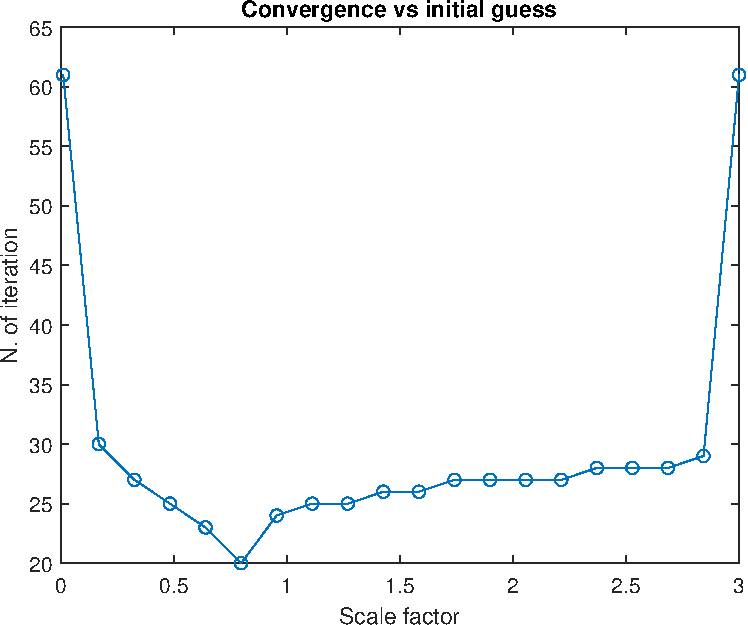
\includegraphics[width=0.9\linewidth]{convergence_vs_initial_guess}
	\caption{Effetto della variazione del parametro iniziale sulla convergenza del metodo. Allontanandosi troppo dalla soluzione iniziale (\texttt{scale factor}=1) il metodo non converge.}
\end{figure}


\section{Conclusioni}

Entrambi i metodi sono validi e permettono di raggiungere il risultato stimando i parametri.

È importante considerare il problema nella forma corretta, considerando i parametri effettivamente linearmente indipendenti e non i differenti elementi circuitali.

Il metodo di Nelder-Mead permette di evitare la derivazione ma porta ad errori medi più elevati. 

Il metodo di Gauss-Newton si mostra più preciso anche se può risultare computazionalmente più costoso. 

Essendo entrambi metodi non lineari, risulta molto importante scegliere il punto iniziale altrimenti il metodo potrebbe non convergere. 

Inoltre, per il metodo di Gauss Newton risulta fondamentale selezionare correttamente i parametri di rilassamento e regolarizzazione per evitare una divergenza del metodo o un costo computazionale più elevato di quanto necessario.

%\pagebreak
\section*{Disponibilità dei dati}

Il materiale è disponibile alla repository online del progetto: \url{https://github.com/mastroalex/respiratory-mechanics}

\subsection*{Codice}

\begin{itemize}
	\item Il codice per l'ottimizzazione con Nelder-Mead a tre parametri è presente nel file \texttt{par\_sys\_id.m}
	\item Il codice per l'ottimizzazione con Nelder-Mead a due parametri è presente nel file \texttt{par\_sys\_id\_two\_param.m}
	\item Il codice per l'ottimizzazione con Gauss-Newton è presente nel file \texttt{par\_sys\_id\_gauss\_newton.m}
\end{itemize}

\raggedbottom

\pagebreak
\printbibliography[title=Riferimenti]
%\section*{References}



